\documentclass[a4paper,11pt,eval]{nsi} 
\usepackage{pifont}
\usepackage{fontawesome5}

%\pagestyle{empty}


\newcounter{exoNum}
\setcounter{exoNum}{0}
%
\newcommand{\exo}[1]
{
	\addtocounter{exoNum}{1}
	{\titlefont\color{UGLiBlue}\Large Exercice\ \theexoNum\ \normalsize{#1}}\smallskip	
}



\begin{document}



\textcolor{UGLiBlue}{Vendredi 22/11/2024}\\
\classe{\premiere spé}
\titre{Evaluation-bilan 2 - Sujet A}
\maketitle
\begin{center}
	Calculatrice interdite
\end{center}

\vspace{.5cm}

\exo{}\bareme{4 pts}\\
Les courbes ci-dessous sont des paraboles représentant chacune une fonction trinôme\\ $f:x\mapsto ax^2+bx+c$ dans un reprère orthogonal.\\[.5em]
Dans chaque cas, donner le signe de $a$ ainsi que le signe du discriminant $\Delta$.\\

\dleft{10cm}{
    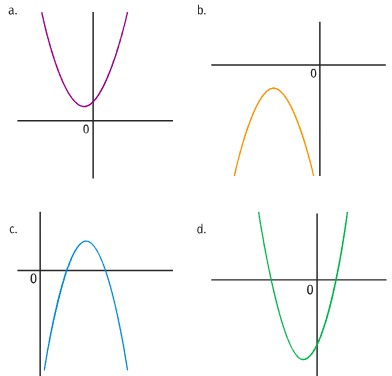
\includegraphics[width=10.5cm]{courbes.jpg}
}
{
    \begin{enumalph}
        \item Signe de $a$ : \dotfill\\[1em]
            Signe de $\Delta$ : \dotfill\\
        \item Signe de $a$ : \dotfill\\[1em]
            Signe de $\Delta$ : \dotfill\\
        \item Signe de $a$ : \dotfill\\[1em]
            Signe de $\Delta$ : \dotfill\\
        \item Signe de $a$ : \dotfill\\[1em]
            Signe de $\Delta$ : \dotfill
    \end{enumalph}
}

\newpage
\exo{}\bareme{10 pts}
\begin{enumerate}
    \item On définit la fonction $f$ sur $\R$ par : $\quad f(x)=-3x^2-2x+1$.
    \begin{enumalph}
        \item Résoudre dans $\R \quad f(x)=0$.
        \item  Résoudre dans $\R \quad f(x)<0$.
        \item Donner, si elle existe, la forme factorisée de $f$. 
    \end{enumalph}
    \carreauxseyes{16}{21.6}
    \item On définit la fonction $g$ sur $\R$ par : $\quad g(x)=2x^2-2x+1$.
    \begin{enumalph}
        \item Résoudre dans $\R \quad g(x)=0$.
        \item  Résoudre dans $\R \quad g(x)>0$.
        \item Donner, si elle existe, la forme factorisée de $g$. 
    \end{enumalph}
    \carreauxseyes{16}{21.6}
\end{enumerate}

\newpage

\exo{}\bareme{6 pts}\\
\dleft{11.5cm}{
    La figure ci-contre représente le logo d'une entreprise.\\
    ABCD est un carré de côté 4 cm. AFKE et KHCG sont des carrés.\\
    La créatrice de ce logo souhaite que l'aire de la surface colorée soit la plus petite possible.\\

    Pour quelle valeur de $x$ la surface colorée a-t-elle la plus petite aire ?\\ Quelle est alors l'aire de cette surface ?
}
{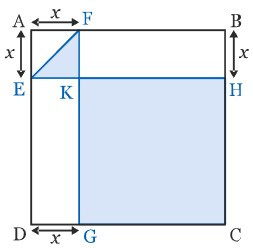
\includegraphics[width=5cm]{logo.jpg}}
\ding{111} Utilisation d'une aide.\\[.5em]
\carreauxseyes{16.8}{19.2}

\subsection*{NOM, Prénom : \dotfill} 
\textit{Pour cet exercice, la calculatrice est autorisée.}\\

\exo{ Sujet A}\bareme{5 pts}\\
$f$ et $g$ sont deux fonctions trinômes du second degré.\\
L'écran de la calculatrice est abîmé et on ne peut pas lire l'expression de $g(x)$ en fonction de $x$.\\[.5em]
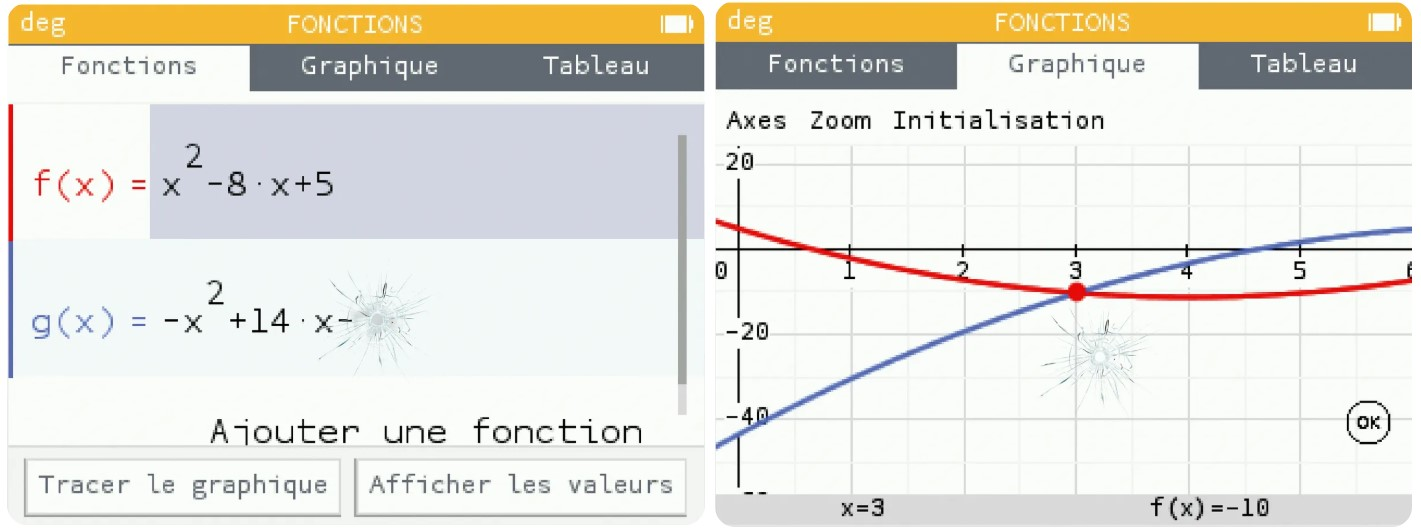
\includegraphics[width=17cm]{calculatrice.jpg}\\[.5em]
Calculer le coefficient manquant dans l'expression de $g(x)$.\\
En déduire par le calcul la deuxième solution de l'équation $f(x)=g(x)$.\\[.5em]
\carreauxseyes{16.8}{13.6}\\
\carreauxseyes{16.8}{25.6}


\end{document}